%# -*- coding: utf-8-unix -*-
%%==================================================
% \addbibresource{bib/qbook.bib}
\chapter{端到端文字识别(Scene Text Spotting)}


2018年以前,关于Scene Text Spotting的论文\cite{liu2018fots},主要集中在解决旋转文本的端到端识别问题,几乎没有论文解决曲形文本端到端识别的问题。
自从发表在ECCV2018中的论文,MaskTextSpotter\cite{lyu2018mask},开始试图解决曲形文本端到端识别的问题以来,大量的工作开始致力于该问题的研究,如
\cite{lyu2018mask,liao2019mask,Feng_2019_ICCV,Xing_2019_ICCV,qin2019towards,wang2019all,liu2020abcnet,qiao2020text}。自此,
端到端文本识别方法在理论上能够解决任意形状文本识别的问题。在以下表述中以“任意形状文本端到端识别方法”来统称既能处理多方向又能处理曲形文本的端到端文本识别
方法。

\begin{figure}[H]
    \centering
    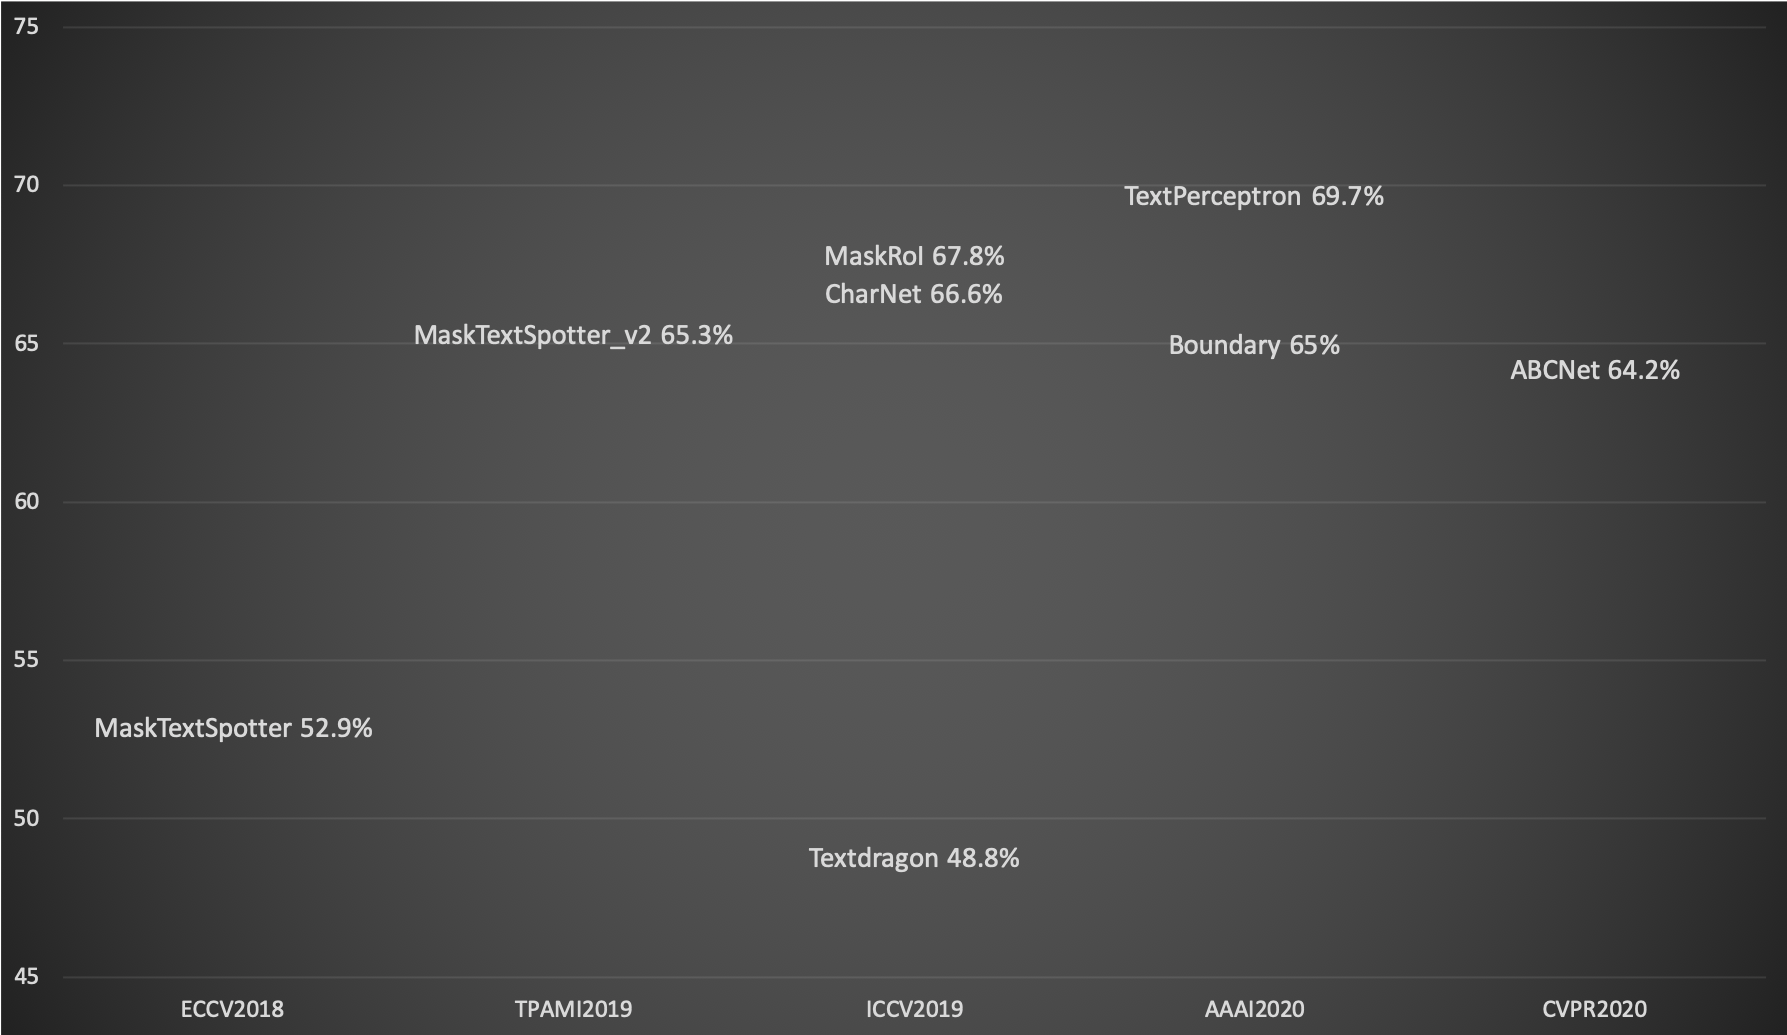
\includegraphics[width=.98\textwidth]{figure/spotting/trends.png} 
    \caption{2018年到2020年3月期间,曲形文本端到端文本识别方法在TotalText上的性能。} 
    \label{spotting_tends} 
\end{figure}

首先,我们从问题的角度出发,概述各种任意形状文本端到端识别方法之间的关系。然后将从方法,实验结果,该方法的优缺点等方面来分别探讨各种方法,这些方法包括:
MaskTextSpotter\cite{lyu2018mask,liao2019mask}、TextDragon\cite{Feng_2019_ICCV}、CharNet\cite{Xing_2019_ICCV}、
MaskRoI\cite{qin2019towards}、Boundary\cite{wang2019all}、TextPerceptron\cite{qiao2020text}以及ABCNet\cite{liu2020abcnet}。
最后,进一步总结归纳以上方法的特点。



% \section{任意形状文本端到端识别方法的发展脉络}



\section{各种任意形状文本端到端识别方法介绍}
\subsection{MaskTextSpotter (ECCV2018)}
\subsubsection{MaskTextSpotter网络结构}
MaskTextSpotter作为首个任意形状文本端到端识别方法,其思路是将每个文字字符作为一个类别进行检测。其网络框架如图\ref{masktextspotter_framework}所示,网络
主体部分与MaskRCNN\cite{he2017mask}一致。由于常规的MaskRCNN网络(分割分支进行1通道的分割,表示是否为文字两个类别)只能完成文字检测任务,无法进行文字识别,
因此作者将Mask分支设计为37个通道(26个英文字符加上10个数字以及表示是否为字符区域的1通道)加上检测的1个类别共38个类别进行分割,其分割分支如图\ref{masktextspotter_maskbranch}所示。
在测试阶段,检测的1通道能够检测任意形状的文本。根据另外37个通道的分割信息,按照从左到右的顺序连接每个字符,完成识别任务。

\begin{figure}[htb]
    \centering
    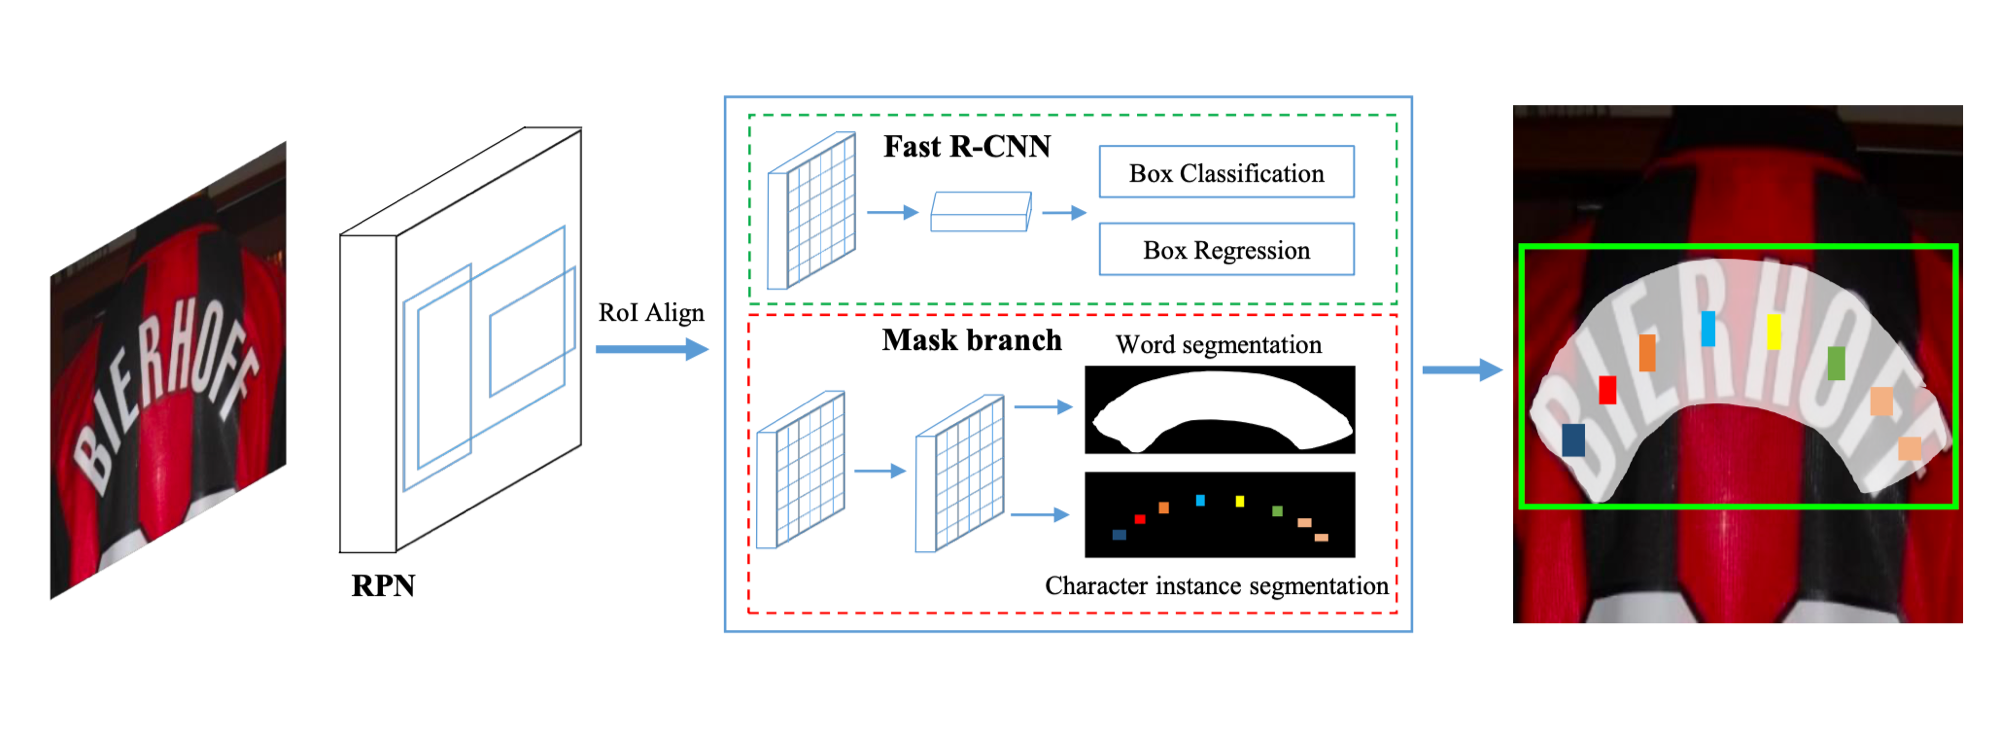
\includegraphics[width=.98\textwidth]{figure/spotting/masktextspotter_framework.png} 
    \caption{MaskTextSpotter框架图。} 
    \label{masktextspotter_framework} 
\end{figure}

\begin{figure}[htb]
    \centering
    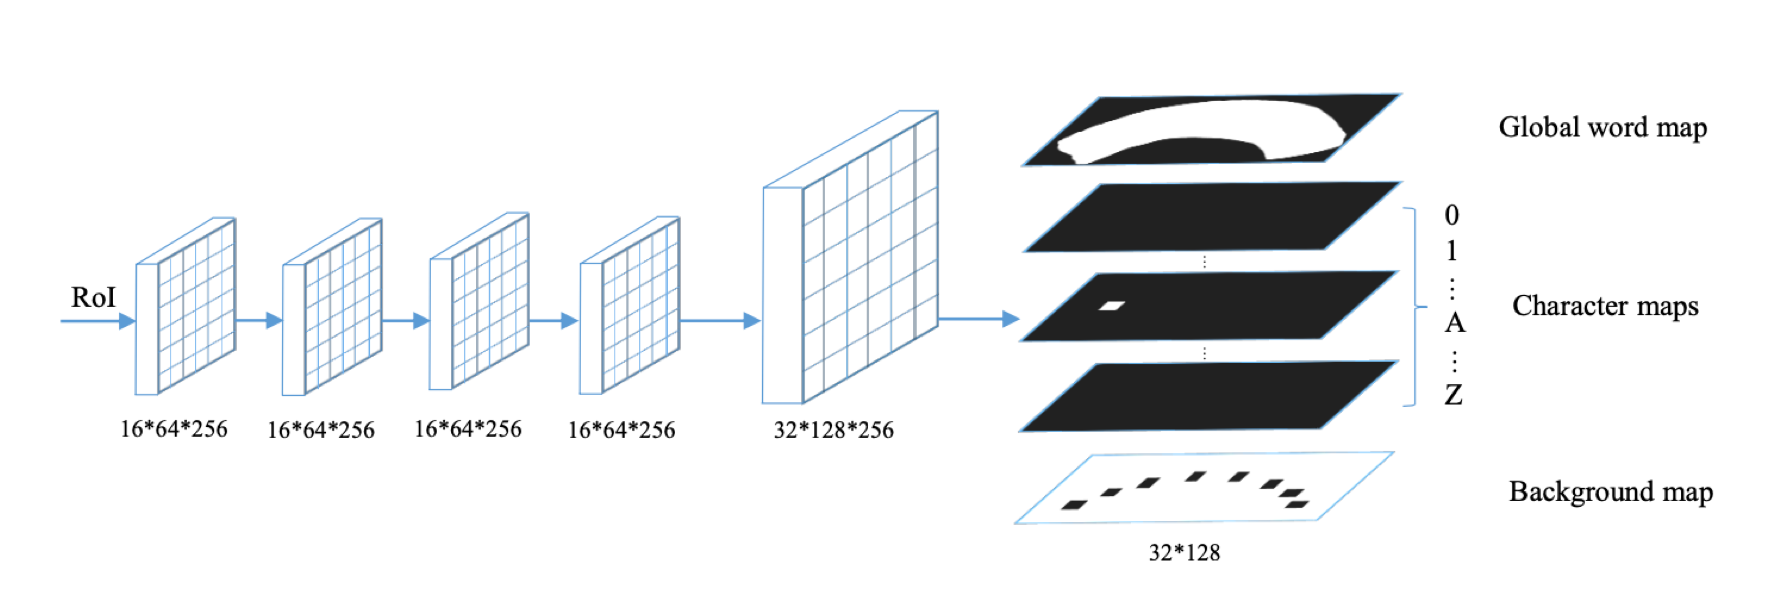
\includegraphics[width=.98\textwidth]{figure/spotting/masktextspotter_maskbranch.png} 
    \caption{MaskTextSpotter的分割分支结构图。} 
    \label{masktextspotter_maskbranch} 
\end{figure}

\subsubsection{MaskTextSpotter实验细节}
MaskTextSpotter的训练过程分为两部分:合成数据集预训练和真实数据集微调阶段。合成数据集使用的是SynthText\cite{gupta2016synthetic},batch size为8,输入图像
以短边为800,保持长宽比进行训练。在真实数据微调阶段,batch size为8,采用多尺度训练的策略,短边分为(600,800,1000)三个尺度进行训练,
使用的数据集有SynthText, ICDAR2013, ICDAR2015, TotalText以及来自\cite{zhong2016deeptext}的1162张图像。

\subsubsection{MaskTextSpotter\_v2网络结构}
由于MaskrTextSpotter中将通过将每个字符作为单独的类别分割出来作为识别结果,这样会导致识别过程中忽略文字的语义特征。基于此,MaskTextSpotter\_v2的主要出发点是将文字
的语义信息融入到识别分支中,最终其网络结构如图\ref{masktextspotter_v2_framework}所示。可以看出,该网络结构和MaskTextspotter相比,在识别分支加入了序列识别分支。
其识别分支具体结构如图\ref{masktextspotter_v2_recog}所示。

识别分支由两部分组成:基于字符分割的识别分支和基于序列识别的识别分支。每个识别分支在输出识别结果的同时对识别结果的置信度进行打分,最终的识别结果取置信度较高的分支的识别结果。
\begin{figure}[htb]
    \centering
    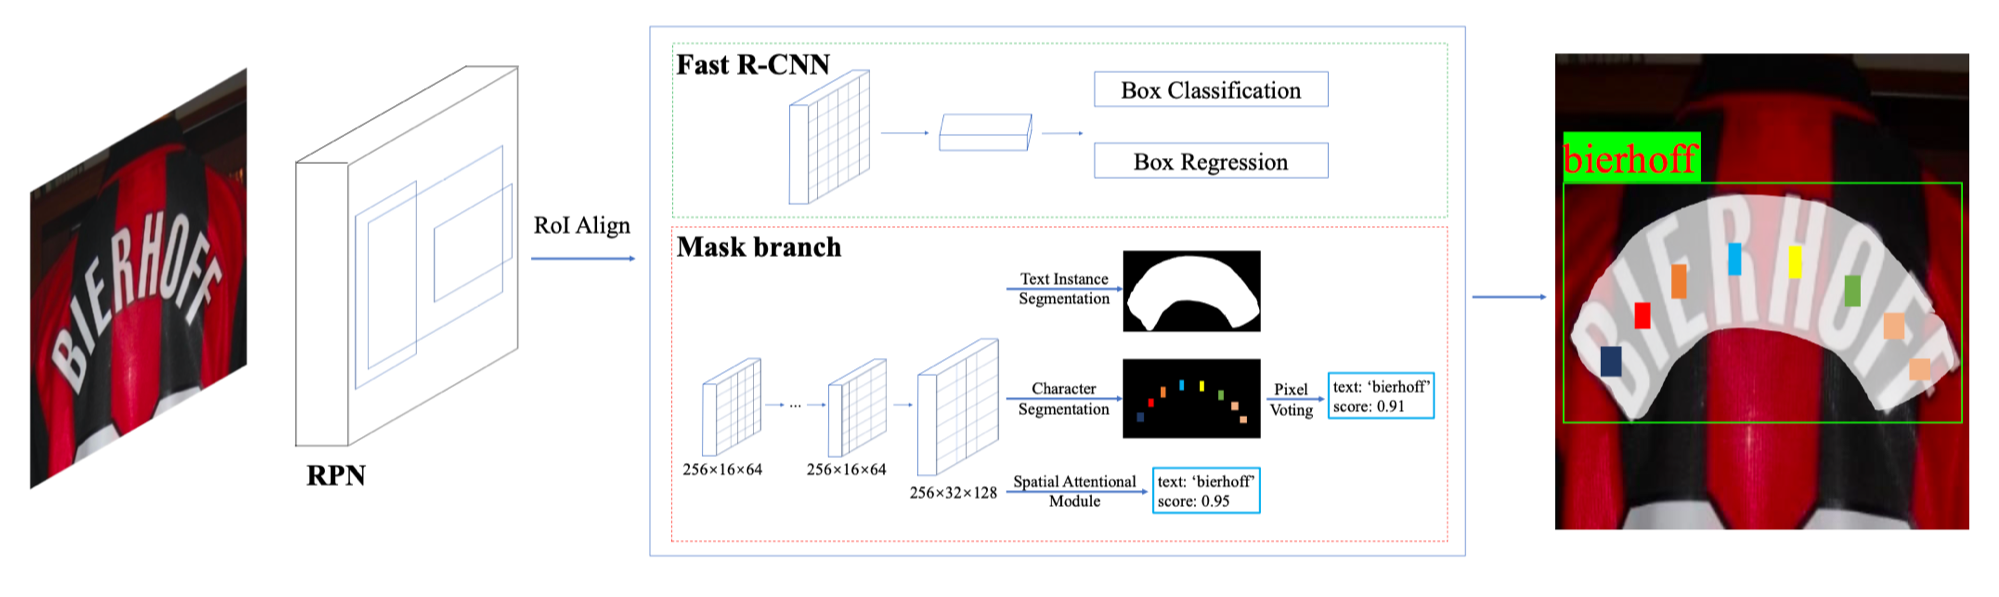
\includegraphics[width=.98\textwidth]{figure/spotting/masktextspotter_v2_framework.png} 
    \caption{MaskTextSpotter\_v2框架图。} 
    \label{masktextspotter_v2_framework} 
\end{figure}

\begin{figure}[htb]
    \centering
    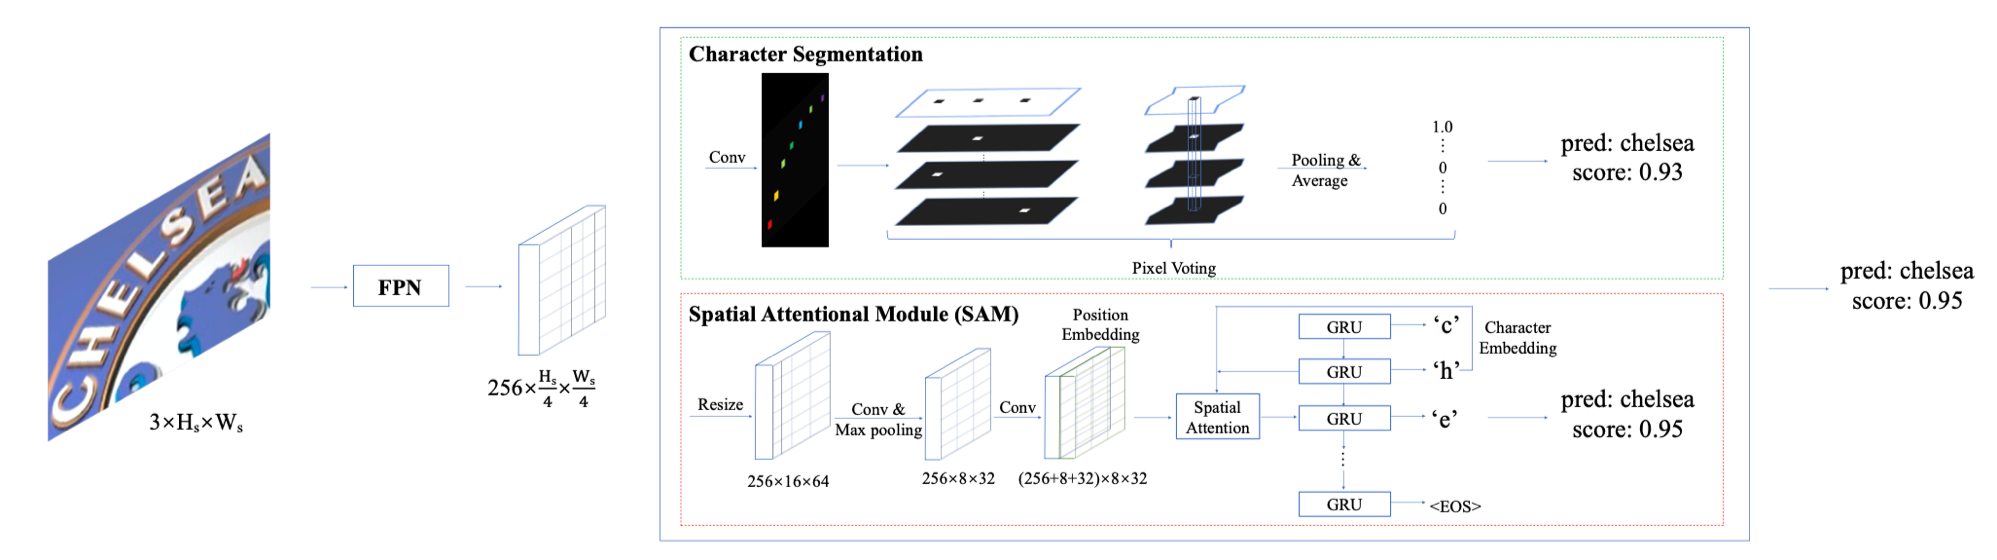
\includegraphics[width=.98\textwidth]{figure/spotting/masktextspotter_v2_recog.png} 
    \caption{MaskTextSpotter\_v2识别分支结构图。} 
    \label{masktextspotter_v2_recog} 
\end{figure}

\subsubsection{MaskTextSpotter\_v2实验细节}
MaskTextSpotter的训练过程分为两部分:合成数据集预训练和真实数据集微调阶段。
合成数据集使用的是SynthText\cite{gupta2016synthetic},batch size为8,输入图像
以短边为800,保持长宽比,学习率从0.001开始,第100k,200k次下降0.1,训练270k步。
在真实数据微调阶段,batch size为8,采用多尺度训练的策略,短边分为(600,800,1000,1200,1400)三个尺度进行训练,
使用的数据集有SynthText, ICDAR2013, ICDAR2015, TotalText以及来自\cite{zhong2016deeptext}的1162张图像。
学习率从0.001开始,第100k下降0.1,训练150k步。

\subsection{TextDragon (ICCV2019)}
虽然MaskTextSpotter能够进行任意形状文本端到端的识别,但是数据集字符级别的标注的要求使得网络的训练比较昂贵。TextDragon
意在只使用单词级别的标注来设计任意形状文本端到端识别系统。
\subsubsection{TextDragon网络结构}
TextDragon对任意形状文本的表示方式主要来自于文字检测方法TextSnake\cite{long2018textsnake},也就是将任意形状
的文本表示为一系列的带方向正方形。然后从属于同一文本实例的带方向正方形中聚合,采样一个子集形成文本区域。基于该子集的带方向正方形,
则有:
1)从这些带方向正方形中提取文字边界点来表示检测结果,2)对每个正方形区域的特征进行字符分类,通过CTC解码成文本字符串。
TextDragon的网络结构如图\ref{textdragon_framework}所示。

具体地,文字的表示方法如图\ref{textdragon_representation}所示。文本实例由文本的中心线、正方形边长以及正方形旋转方向构成。
在测试阶段,推理过程如下:1)通过文本中心线来获取每个文本实例大致区域;2)在每个文本实例的中心线上获得所有的预测的带方向正方形,
并保留这些IOU大于0.5,旋转角度差小于45度的正方形区域;3)根据其位置将这些保留的正方形进行排序,形成表示该文本区域的正方形子集。
4)最终通过RoISlide从这些矫正后的文本区域中获取特征,进行字符串识别,而文本边界由正方形子集形成的边界点构成。
\begin{figure}[htb]
    \centering
    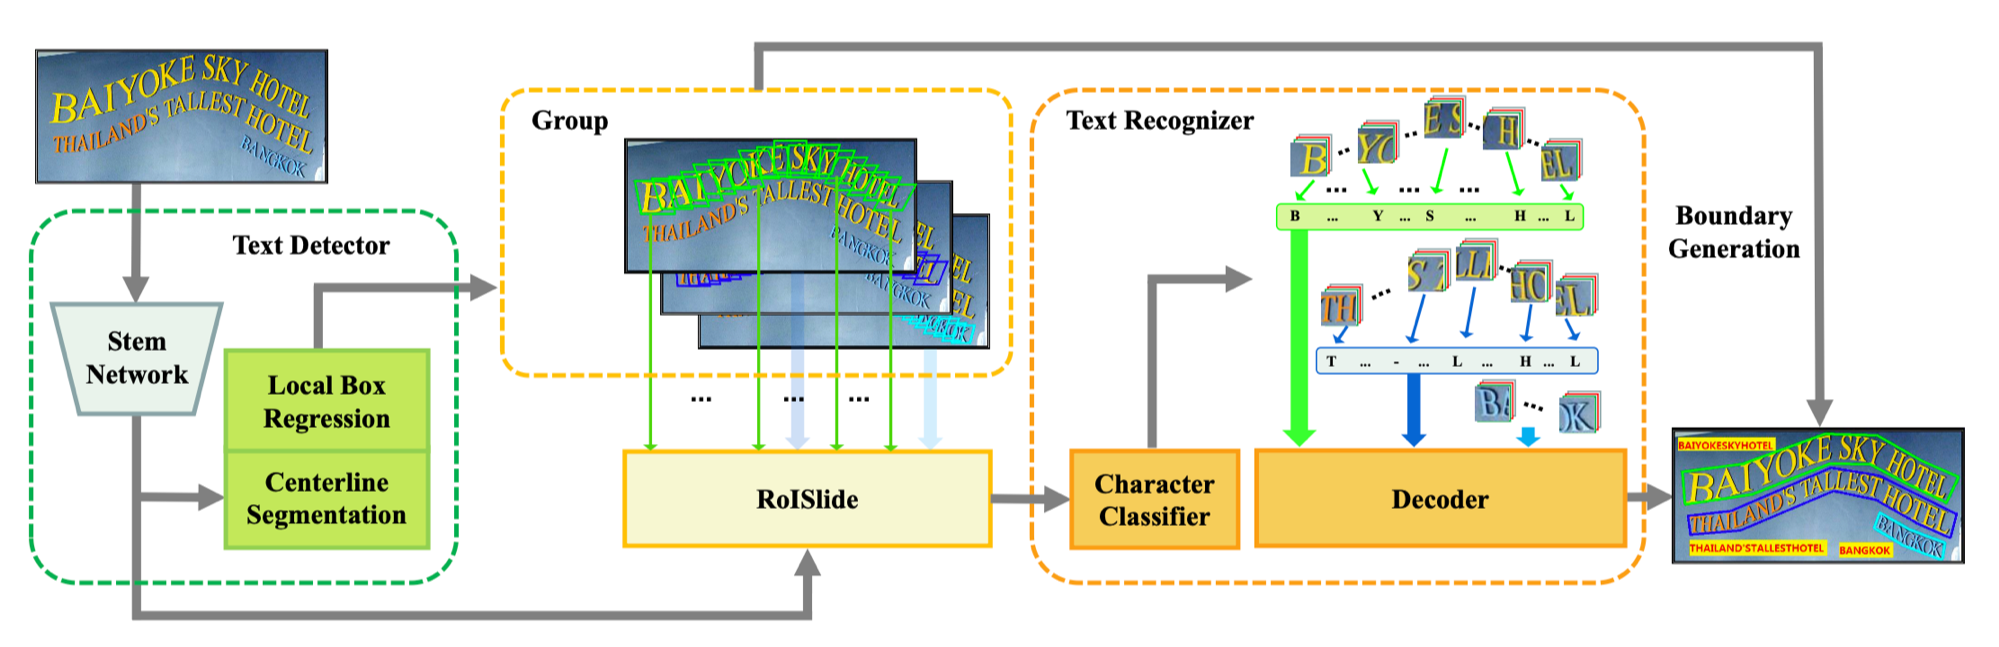
\includegraphics[width=.98\textwidth]{figure/spotting/textdragon_framework.png} 
    \caption{TextDragon框架图。} 
    \label{textdragon_framework} 
\end{figure}

\begin{figure}[htb]
    \centering
    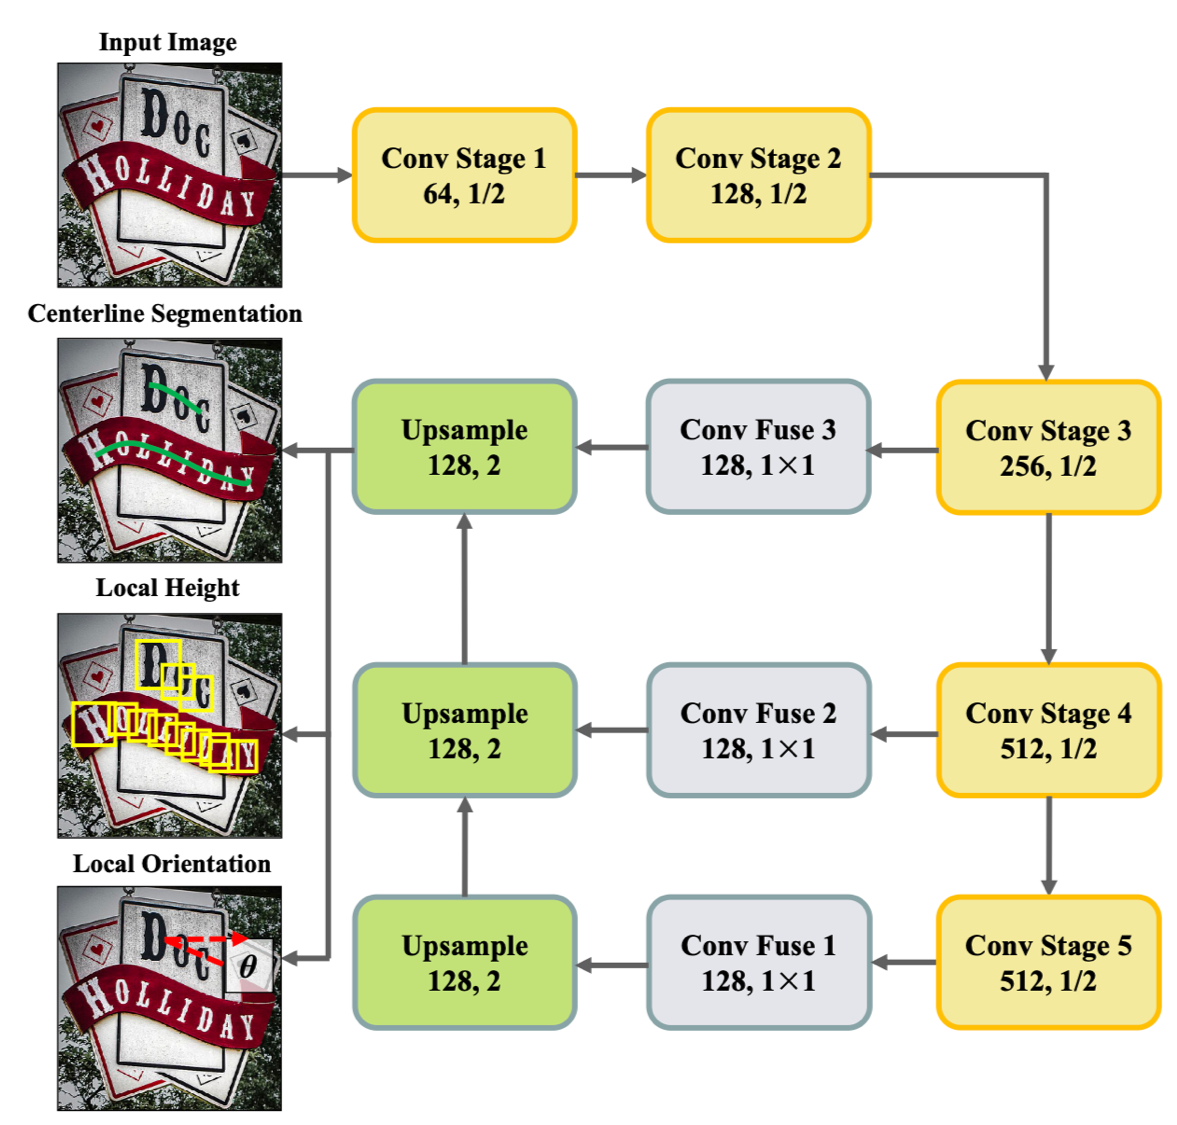
\includegraphics[width=.7\textwidth]{figure/spotting/textdragon_representation.png} 
    \caption{TextDragon文本实例表示方法。} 
    \label{textdragon_representation} 
\end{figure}

\subsubsection{TextDragon实验细节}
TextDragon的训练过程分为两部分:合成数据集预训练和真实数据集微调阶段。
合成数据集使用的是SynthText,输入图像大小为512*512,学习率为0.01,训练600k步。
在真实数据微调阶段,输入图像大小为512*512,数据集为相对应数据集的训练集,学习率为0.001,训练120k步。

\subsection{CharNet (ICCV2019)}
CharNet与TextDragon一样是在任意形状文本端到端识别算法只有MaskTextSpotter的背景下出现的方法。他的主要出发点是:当前端到端识别的方法中,
都是two stage的(这里two stage是指检测网络得到检测结果,再根据检测结果利用RoI操作获取特征进行识别),作者认为two stage中RoI提取很难提取
准确(主要是检测存在误差),并且two stage过程繁琐,不便使用。因此,作者想设计一个single stage的网络,同时输出文本实例的检测和识别结果。
\subsubsection{CharNet网络结构}
CharNet在核心问题上和MaskTextSpotter一致,都是通过字符级别的分割解决任意形状文本的识别问题。MaskTextSpotter是在RoI内进行分割,而CharNet是在
全图进行字符级别的分割。那么,CharNet就剩下最后一个需要解决的问题:如何将分割出的字符group成为一个文本区域?
如CharNet网络结构图\ref{charnet_framework}所示,其Detection Branch的作用便是预测一些信息来将分割出的字符聚合成字符串。
对于多方向文本,其Detection Branch的表示方法为EAST\cite{zhou2017east}的表示方式,利用预测的四边形框的IoU聚合每个字符为字符串。
对于曲形文本,其Detection Branch的表示方法为TextField\cite{xu2019textfield}的表示方法。
\begin{figure}[htb]
    \centering
    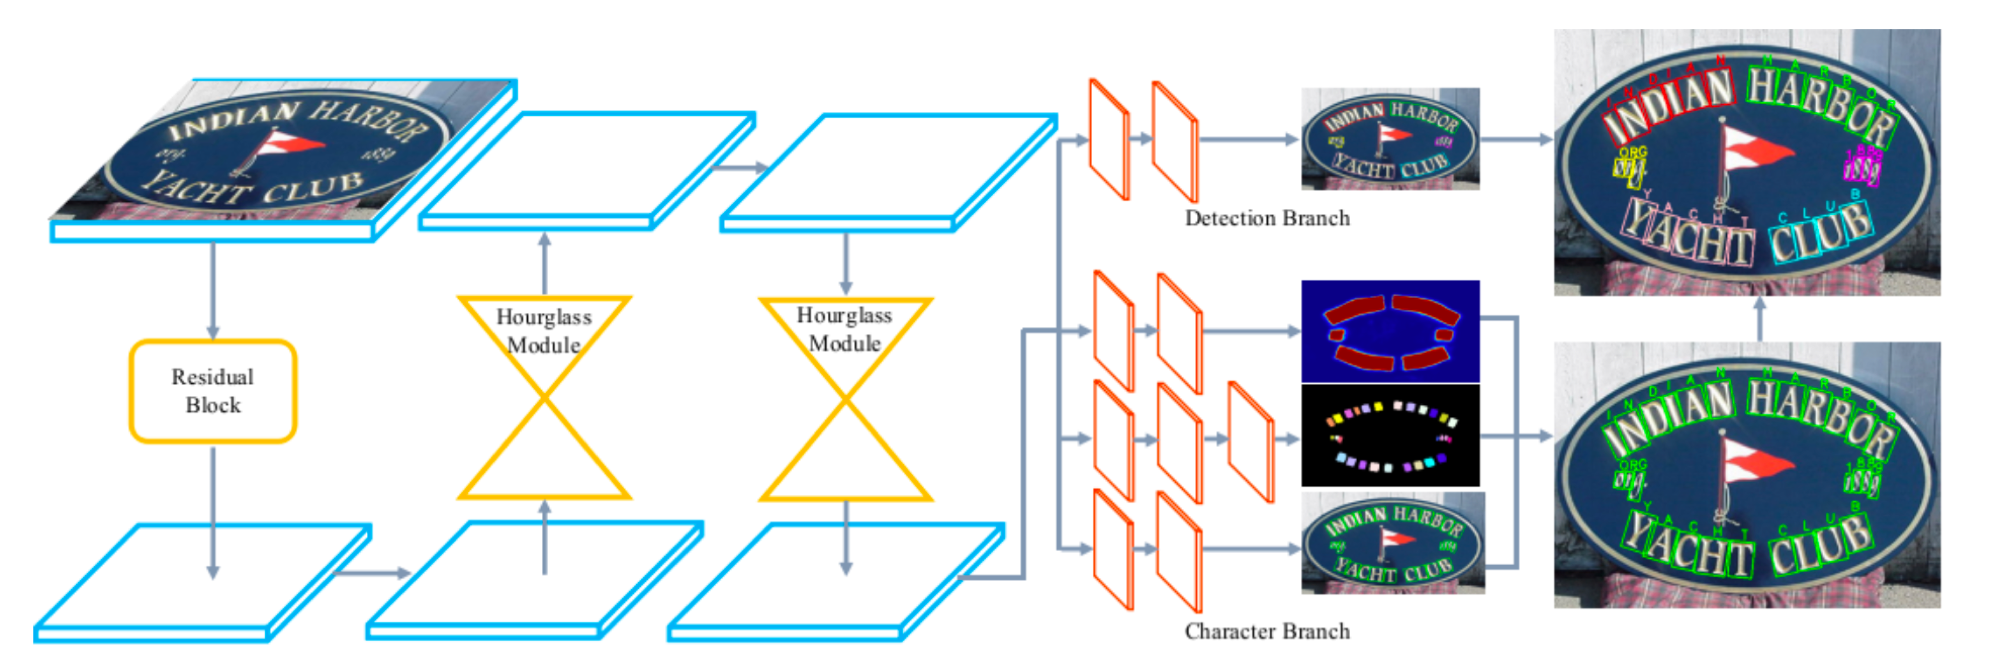
\includegraphics[width=.98\textwidth]{figure/spotting/charnet_framework.png} 
    \caption{CharNet框架图。} 
    \label{charnet_framework} 
\end{figure}

\subsubsection{CharNet实验细节}
CharNet的训练过程分为两部分:合成数据集预训练和真实数据集微调阶段。
合成数据集使用的是SynthText,batch size为32,学习率为0.0002,数据集迭代5 epochs。
在真实数据微调阶段,数据集为相对应数据集的训练集,学习率为0.002,分三步进行迭代训练,三步训练回合分别为100,400,800epochs。
这里每步迭代训练是指:利用先前的模型获得训练集的字符级别标注(检测框),过滤出正确的字符级别标注来训练模型,迭代n(100,400或800)个epochs。

\subsection{MaskRoI (ICCV2019)}
MaskRoI与CharNet以及TextDragon是同时期文章,该方法不需要字符级别的标注,同时不需要将任意形状文本矫正为水平文本进行识别。
\subsubsection{MaskRoI网络结构}
如图\ref{maskroi_framework}所示,MaskRoI和MaskTextSpotter一样,也是基于MaskRCNN框架进行改进的。识别分支采用基于attention的序列识别方案。
为了解决任意形状文本的RoI容易采样到背景或者相邻文本特征的问题,在进行序列识别之前,进行了特征过滤操作。该操作就是将文本实例分割图和RoI的特征进行相乘。

\begin{figure}[htb]
    \centering
    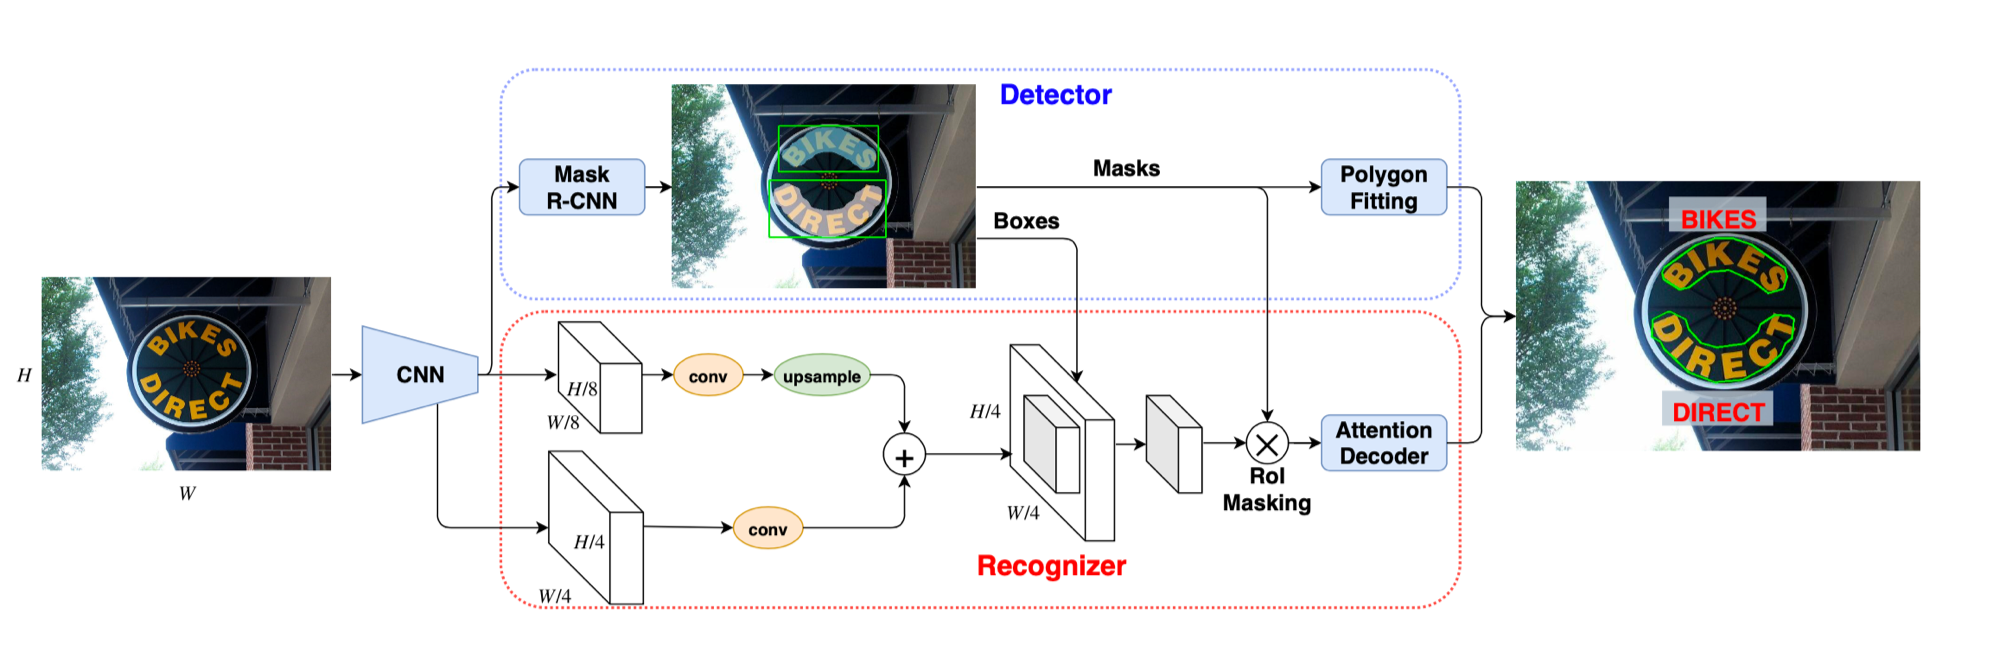
\includegraphics[width=.98\textwidth]{figure/spotting/maskroi_framework.png} 
    \caption{MaskRoI框架图。} 
    \label{maskroi_framework} 
\end{figure}

\subsubsection{MaskRoI实验细节}
MaskRoI采用一步训练的方式,数据集包括SynthText,ICDAR2015,COCOText,ICDAR-MLT,TotalText以及网络收集的通过Google OCR Api标注的30k张图像。
采用多尺度训练的策略,短边为480到800之间。

\subsection{Boundary (AAAI2020)}
Boundary\cite{wang2019all}和基于分割的方法得到任意形状文本的边界不同,该文章通过回归的方式获得任意形状文本的边界,从而避免负责的后处理过程使得检测识别两个过程完全端到端可训练。
\subsubsection{Boundary网络结构}
Boundary的网络结构如图\ref{boundary_framework}所示:网络整体基于FPN网络,首先检测出文本的长方形包围盒,提取该长方形内的特征(这样相当于将文本在角度上进行了归一化,使得边界点的回归更为准确);
然后检测文本的边界点,最后通过Arbitrary RoIAlign将曲形文本矫正为水平文本特征进行识别。
\begin{figure}[H]
    \centering
    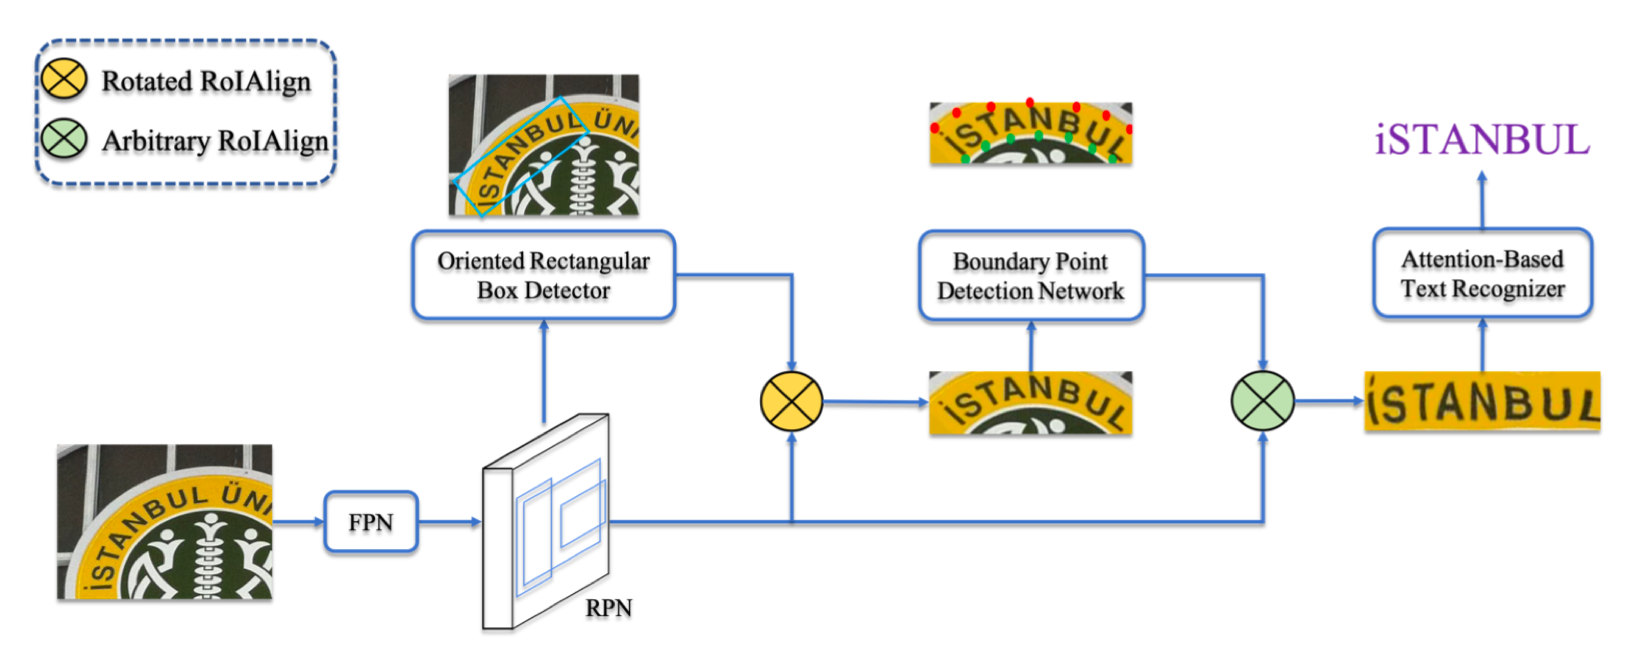
\includegraphics[width=.98\textwidth]{figure/spotting/boundary_framework.png} 
    \caption{Boundary框架图。} 
    \label{boundary_framework} 
\end{figure}

Boundary详细的回归细节如图\ref{boundary_regress}所示:准确回归出文本边界点的重要细节在于,在(b)处将文本的方向信息进行了归一化(即将文本旋转为水平进行边界点的检测),这样使得边界点的分布更为稳定。
另外,文章中并不是直接预测边界点的坐标,而是在预设的anchor points基础上进行边界点的回归,这样同样可以简化边界点的回归任务。
\begin{figure}[H]
    \centering
    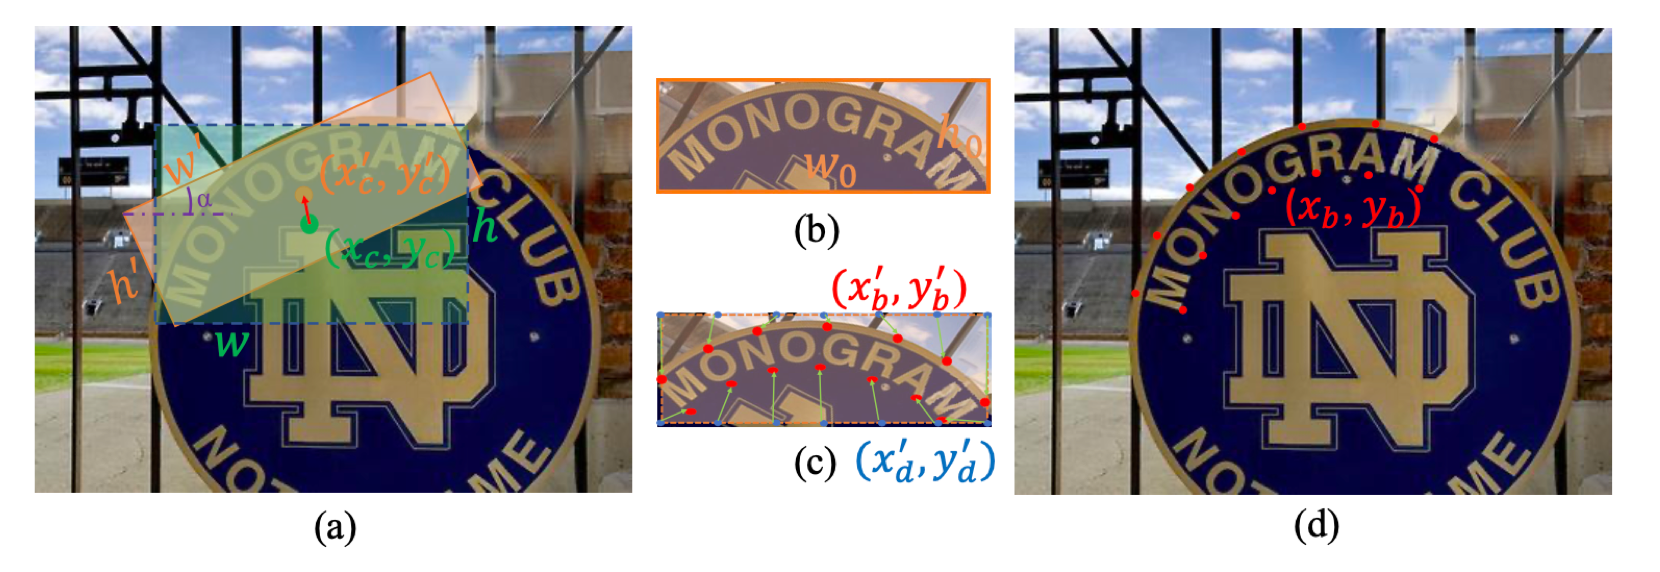
\includegraphics[width=.98\textwidth]{figure/spotting/boundary_regress.png} 
    \caption{Boundary回归过程:(a)回归出文本的带方向的长方形包围盒;(b)归一化文本角度;(c)从anchor points处回归到boundary points。} 
    \label{boundary_regress} 
\end{figure}

\subsection{TextPerceptron (AAAI2020)}
TextPerceptron的主体思路也是文本实例边界点检测+TPS+序列识别。和Boundary不同之处在于文本边检点检测过程,具体地说,是通过文本实例的几何属性和后处理得到
边界点。
\subsubsection{TextPerceptron网络结构}
TextPerceptron的网络结构如图\ref{textperceptron_framework}所示。边界点的检测是基于分割的方法,预测的文本实例的几何属性包括:1)文本上下边界;2)文本实例的开端;
3)文本实例的结尾;4)文本实例的中间区域;5)开端以及结尾处的角点回归;6)文本中心区域的边界点回归。其中5)和6)的标签定义如图\ref{textperceptron_label}所示。
\begin{figure}[htb]
    \centering
    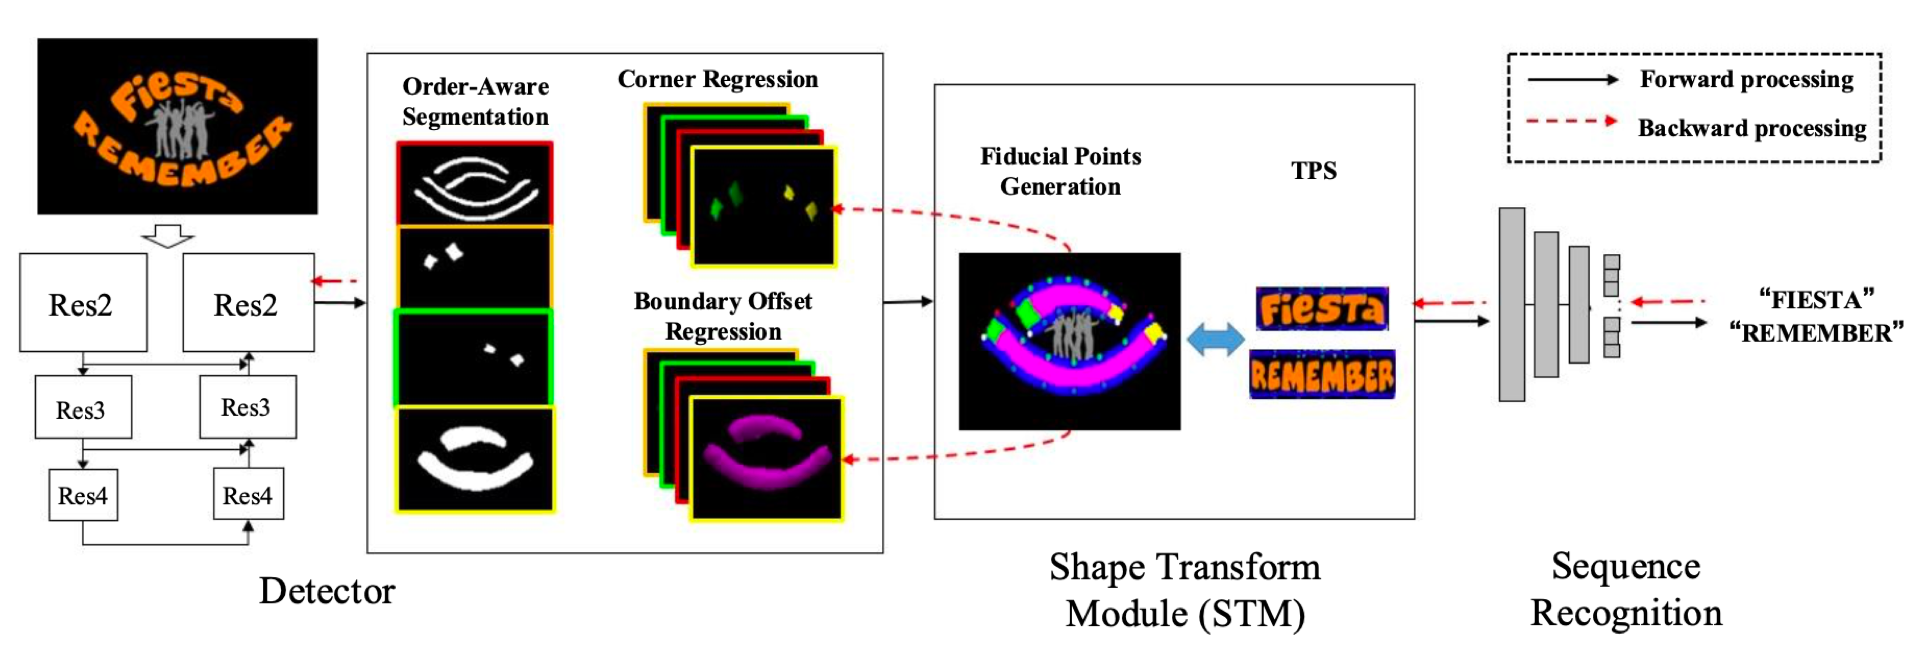
\includegraphics[width=.98\textwidth]{figure/spotting/textperceptron_framework.png} 
    \caption{TextPerceptron框架图。} 
    \label{textperceptron_framework} 
\end{figure}

\begin{figure}[htb]
    \centering
    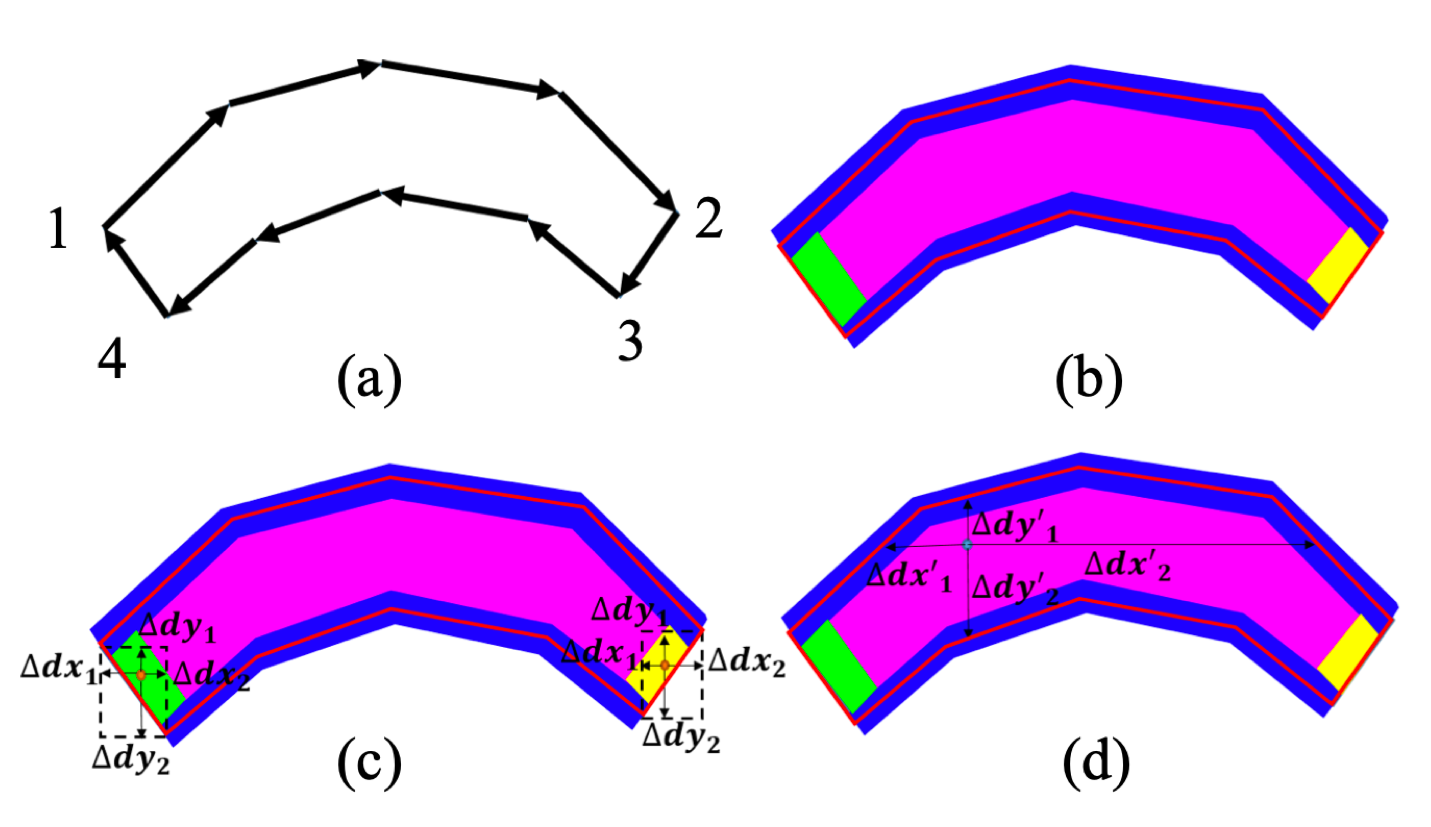
\includegraphics[width=.8\textwidth]{figure/spotting/textperceptron_label.png} 
    \caption{TextPerceptron 角点和边界点回归的定义。} 
    \label{textperceptron_label} 
\end{figure}

\subsubsection{TextPerceptron边界点获取过程}
根据预测的文本实例的几何属性,后处理得到边界点的过程如下:
1)根据中心区域和开端以及结尾的匹配程度可以获得开端、结尾匹配对,上下边界可以用于区分相邻的文本实例;
2)在开端、结尾分割图处获取文本实例的4个角点;
3)如图\ref{textperceptron_process}所示,获得较长边的角点对的中心点,作垂线,获得该点对所处边界的交点作为一个边界点,以此类推,获得所有边界点。
\begin{figure}[htb]
    \centering
    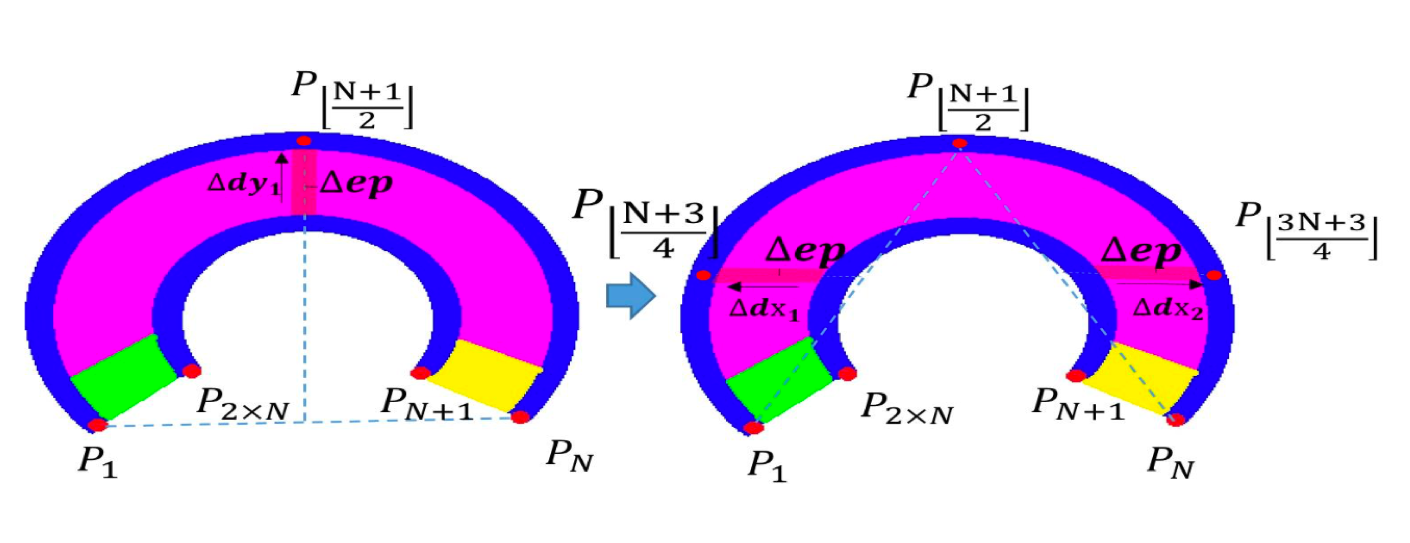
\includegraphics[width=.8\textwidth]{figure/spotting/textperceptron_process.png} 
    \caption{TextPerceptron后处理过程。} 
    \label{textperceptron_process} 
\end{figure}

\subsubsection{TextPerceptron实验细节}
TextPerceptron分为3个阶段,1)训练检测分支,在SynthText上以学习率0.002训练5 epochs;2)训练识别分支,在SynthText上以学习率0.002训练5 epochs;
3)检测识别联合训练,在各自训练集上以学习率0.001训练80 epochs,每20 epochs学习率乘以0.1。


\subsection{ABCNet (CVPR2020)}
ABCNet的主体思路也是文本实例边界点检测+TPS+序列识别。边界点的检测采样回归的方法,和Boundary不同的是,检测部分采用anchor-free的方法。论文的框架主要基于FCOS\cite{tian2019fcos}上进行改进。
\subsubsection{ABCNet网络结构}
ABCNet采用贝塞尔曲线来表示文本实例的边界,贝塞尔曲线描述效果如图\ref{abcnet_basier}所示。网络框架如图\ref{abcnet_framework}所示,FCOS采用密集预测的方式。从代码中可以看出,检测部分的预测信息包括:
1)每个bbox的得分;2)中心区域预测;3)bbox回归;4)贝塞尔曲线控制点预测。
获得贝塞尔曲线后,
\begin{figure}[htb]
    \centering
    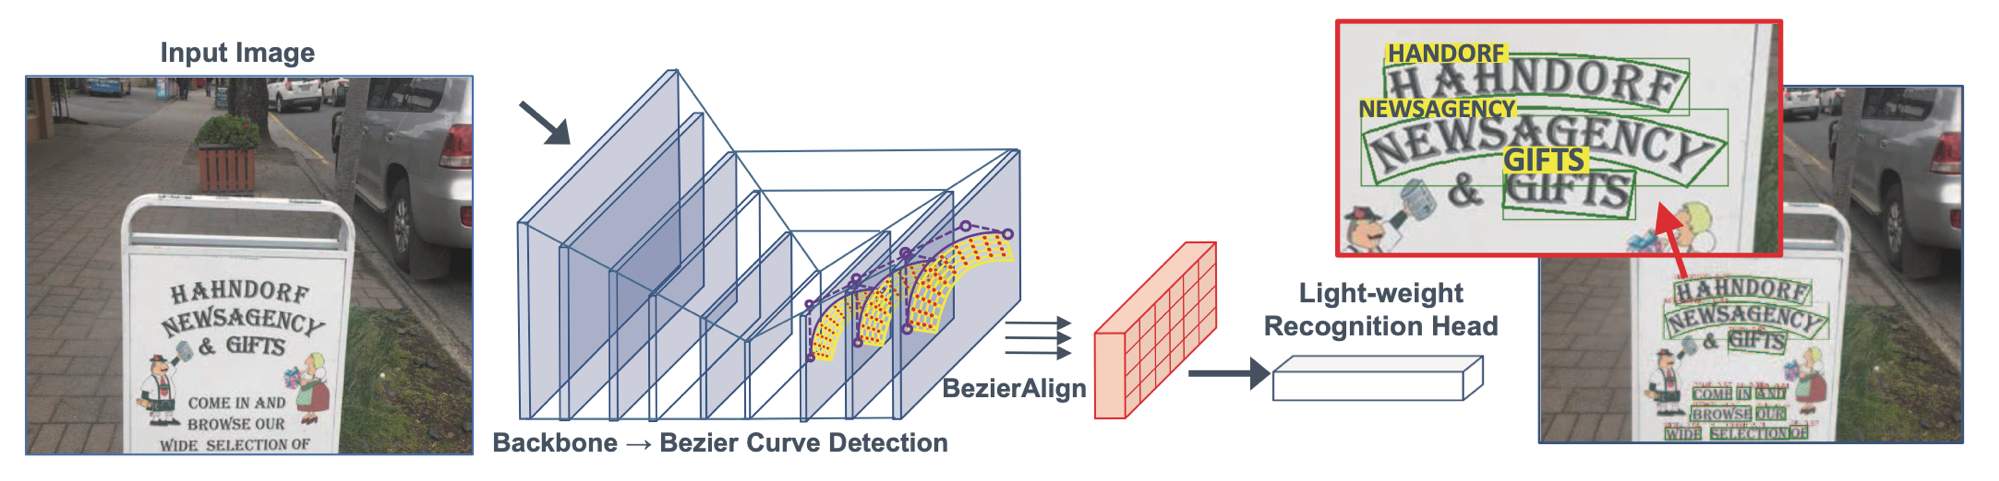
\includegraphics[width=.98\textwidth]{figure/spotting/abcnet_framework.png} 
    \caption{ABCNet框架图。} 
    \label{abcnet_framework} 
\end{figure}

\begin{figure}[htb]
    \centering
    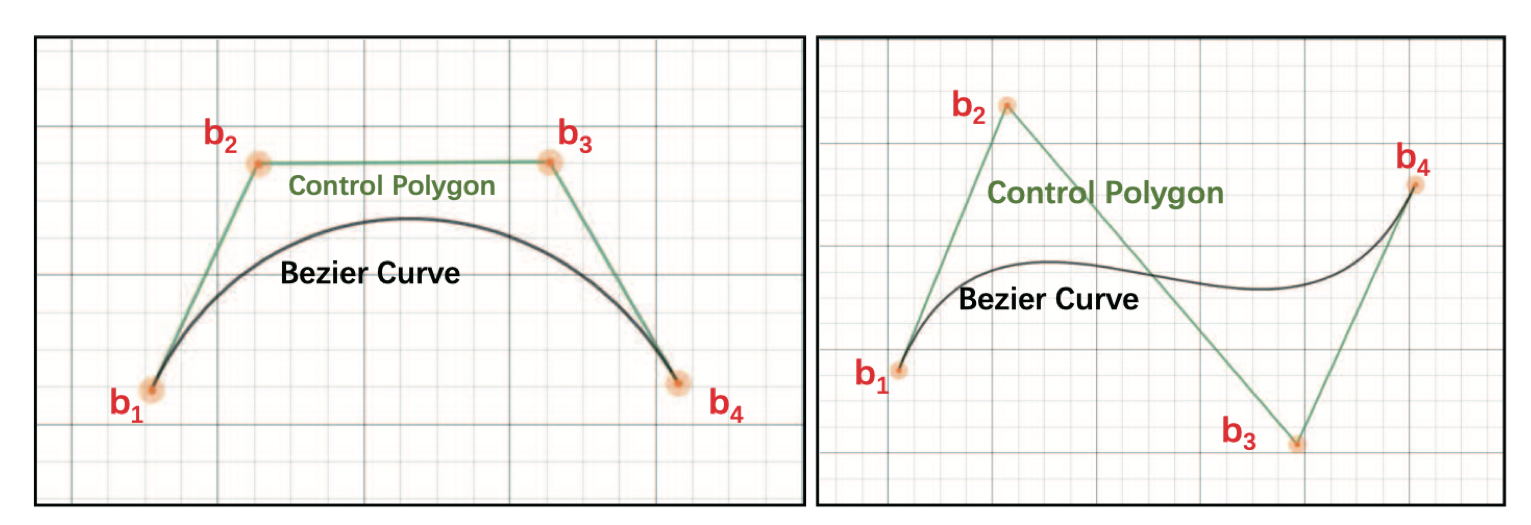
\includegraphics[width=.98\textwidth]{figure/spotting/abcnet_basier.png} 
    \caption{贝塞尔曲线。} 
    \label{abcnet_basier} 
\end{figure}

贝塞尔曲线获得的边界如图\ref{abcnet_sample}所示。
\begin{figure}[htb]
    \centering
    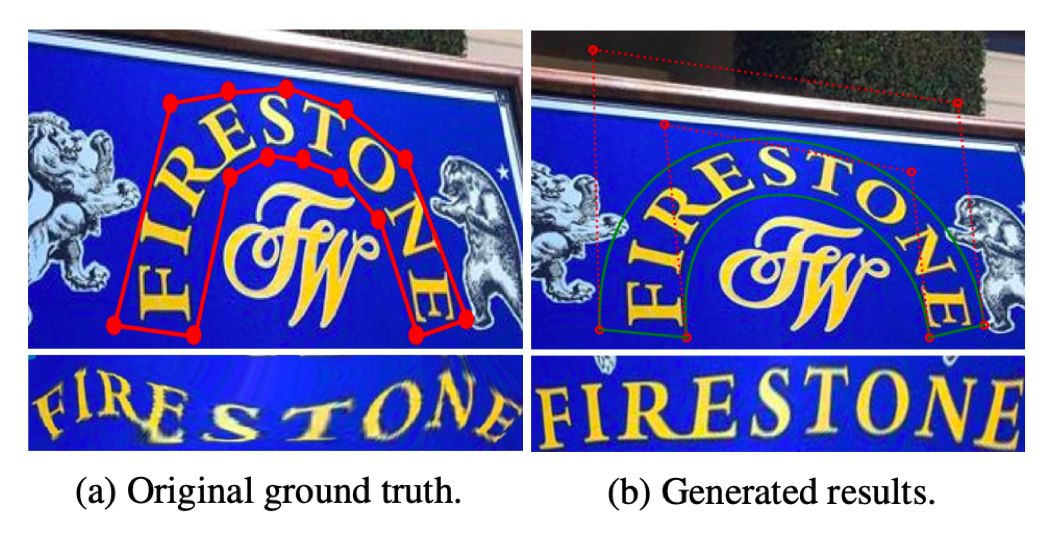
\includegraphics[width=.98\textwidth]{figure/spotting/abcnet_sample.png} 
    \caption{贝塞尔曲线。} 
    \label{abcnet_sample} 
\end{figure}

\subsubsection{ABCNet实验细节}
TextPerceptron分为2个阶段:1)合成的150k合成数据集,15k的COCOText,7k的ICDAR-MLT预训练;2)相应的训练集训练。

% \section{任意形状文本端到端识别方法的总结}
